%
% File acl2018.tex
%
%% Based on the style files for ACL-2017, with some changes, which were, in turn,
%% Based on the style files for ACL-2015, with some improvements
%%  taken from the NAACL-2016 style
%% Based on the style files for ACL-2014, which were, in turn,
%% based on ACL-2013, ACL-2012, ACL-2011, ACL-2010, ACL-IJCNLP-2009,
%% EACL-2009, IJCNLP-2008...
%% Based on the style files for EACL 2006 by 
%%e.agirre@ehu.es or Sergi.Balari@uab.es
%% and that of ACL 08 by Joakim Nivre and Noah Smith

\documentclass[11pt,a4paper]{article}
\usepackage[hyperref]{acl2019}
\usepackage{times}
\usepackage{latexsym}
\usepackage{url}
\usepackage{graphicx}
\usepackage{booktabs}
\usepackage{bm}
\usepackage{amsfonts}
\usepackage{amsmath}
\DeclareMathOperator*{\argmax}{arg\,max}
\DeclareMathOperator*{\argmin}{arg\,min}

\aclfinalcopy % Uncomment this line for the final submission
%\def\aclpaperid{***} %  Enter the acl Paper ID here

%\setlength\titlebox{5cm}
% You can expand the titlebox if you need extra space
% to show all the authors. Please do not make the titlebox
% smaller than 5cm (the original size); we will check this
% in the camera-ready version and ask you to change it back.

\newcommand\BibTeX{B{\sc ib}\TeX}

\newcommand{\dpcomment}[1]{\textcolor{green}{[#1 --deric]}}
\newcommand{\jbcomment}[1]{\textcolor{orange}{[#1 --josh]}}

\title{Syntactically Informed Natural Language Inference}

\author{
  Deric Pang \quad
  Joshua Bean \\
  Paul G. Allen School of Computer Science \& Engineering \\
  University of Washington \\
  Seattle, WA, USA \\
  {\tt \{dericp, jbean96\}@cs.washington.edu} \\
}

\date{}

\begin{document}
\maketitle
\begin{abstract}
We demonstrate the importance of syntactic information in semantic models by extending the
decomposable attention model \citep{Parikh2016-em} for natural language inference
to use syntactic features.
By pipelining the hidden states of a neural syntax parser into the decomposable
attention model, we achieve greater performance on the SciTail dataset
\citep{Khot2018-th} than what is gained by
using contextual embeddings like ELMo \citep{Peters2018-fz}.
\end{abstract}

\section{Introduction}

Natural language inference (NLI) is the task of characterizing entailment and
contradiction relationships between texts. We improve NLI models by adding syntactic
features into existing models.

In general, most NLI tasks are formulated as characterizing the relationship
between a pair of sequences---a premise and a hypothesis. An NLI model should
predict whether the hypothesis is entailed by the premise, contradicts the
premise, or is neutral to the premise.

We extend the decomposable attention (DA) model by \citet{Parikh2016-em}
incorporating syntactic features.
\dpcomment{Include brief summary of contributions here.}
The DA model obtained state-of-the-art results on the
SNLI \citep{Bowman2015-is} dataset at its time of publication while using
drastically fewer parameters than previous NLI models.
We primarily
evaluate on the domain specific Scitail dataset \citep{Khot2018-th}
for both its smaller size and lack of annotation artifacts when compared to SNLI
\citep{Gururangan2018-lj}.

Our model, \textbf{syntail}, achieves \dpcomment{add number here} better 
test accuracy than the vanilla
DA model and \dpcomment{add number here} better test accuracy than DA with ELMo all
while maintaining the core DA architecture.

\section{Decomposable Attention Model}

The DA model is a simple and easily parallelizable approach to NLI.
We summarize it in this section so we can build upon it later.
The model
decomposes into attend, compare, and aggregate steps.

Let
$\bm{p} = \langle p_1, \dots, p_{\ell_p} \rangle$ and
$\bm{h} = \langle h_1, \dots, h_{\ell_h} \rangle$ where each $p_i, h_i \in \mathbb{R}^d$
is a $d$ dimensional word embedding vector.

\paragraph{Attend.} Compute unnormalized attention weights $e_{ij}$ with
a feed-forward neural network $F$:
\begin{align}
    e_{ij} := F(\bm{p})^\mathsf{T} F(\bm{h}).
\end{align}
Compute the aligned subphrases $\bm{H}i$ and $\bm{P}_j$:
\begin{align}
    \bm{H}_i &:= \sum_{j=1}^{\ell_h}\frac{\exp{(e_{ij})}}
                                        {\sum_{k=1}^{\ell_h}\exp{(e_{ik})}}h_j\,, \notag \\
    \bm{P}_j &:= \sum_{i=1}^{\ell_p}\frac{\exp{(e_{ij})}}
                                        {\sum_{k=1}^{\ell_h}\exp{(e_{ik})}}p_i\
\end{align}
where $\bm{H}_i$ is the weighted sum over $\bm{h}$ that aligns to $p_i$ and vice versa
for $\bm{P}_j$.

\paragraph{Compare.} Compare each $(p_i, \bm{H}_i)$ and $(h_j, \bm{P_}j)$ pairs
with another feed-forward neural network $G$:
\begin{align}
    \bm{v}_{1,i} &:= G([p_i, \bm{H}_i])\quad \forall i \in [1,\ldots, \ell_p]\,, \notag \\
    \bm{v}_{2,j} &:= G([h_j, \bm{P}_j])\quad \forall j \in [1,\ldots, \ell_h]\,.
\end{align}

\paragraph{Aggregate.} Aggregate each set of comparison vectors:
\begin{align}
\bm{v}_{1} = \sum_{i=1}^{\ell_p} \bm{v}_{1,i} \qquad\,, \qquad
\bm{v}_{2} = \sum_{j=1}^{\ell_h}  \bm{v}_{2,j}\,.
\end{align}
and make a prediction with a final feed-forward layer $H$:
\begin{align}
    \hat{\bm{y}} = H([\bm{v}_1, \bm{v}_2]).
\end{align}

\section{Our Model}

The motivation for incorporating syntactic information in an NLI model
can be demonstrated with a simple example. Consider the premise ``Adrian is running
and Alex is swimming." If we present the DA model trained on SNLI with the
hypothesis ``Adrian is swimming," it will confidently predict that this
blatantly incorrect hypothesis is entailed by the premise. Observing
any syntactic parse of
the premise will make it obvious that Adrian is in fact running.

Incorporating syntactic information in semantic tasks has been investigated
before by \dpcomment{add references and discussion}.

Our model, \textbf{syntail}, extends the DA model.
We experiment with features generated by two syntax parsers---the
minimal span-based neural constituency parser \citep{Stern2017-co} and
the deep biaffine attention model for dependency parsing \citep{Dozat2016-gs}. We also experiment
with different methods of incorporating the syntactic features extracted
from these parsers.

\subsection{Extracting Syntactic Information}

The minimal span-based neural constituency parser and the deep biaffine attention
model for dependency parsing both encode the input sequence with an LSTM. Using
this LSTM, we obtain
syntactic features $\bm{s}_i$ for each index $i$ of the input. $\bm{s}_i$ is either
the final hidden state $\bm{r}_i$ of the LSTM at index $i$ or a projected
representation of $\bm{r}_i$.

In the initial 
iteration of the network, syntax is not incorporated until the very last feed-forward 
layer. This means that syntax is not considered when calculating attention between 
the premise and the hypothesis. We speculated that by introducing syntax to the 
network prior to calculating attention we would see better results as the syntax 
would help influence the attention calculations and reveal the most important phrases 
of each input statement.

In the ``V3" model, we perform the same initial step of embedding the premise and 
hypothesis and expanding their dimensions (through a fully-connected layer) prior to 
attention. However, instead of calculating our similarity matrix using solely the 
embedded hypothesis and premise vectors as input, we also provide the encoded syntax 
parses of both inputs. The concatenation of these four vectors is used to derive the 
similarity matrix which is then utilized in the attention computations between the 
premise and hypothesis. \jbcomment{Insert V3.jpg here?}

With the ``V5" model we tried to incorporate the computed syntax of the inputs even 
earlier. Instead of concatenating the encoded syntax parses with the embedded inputs 
and using that as input for the computation of the similarity matrix, we concatenated 
the syntax parses with their respective inputs and passed that through the first 
fully-connected layer. The two resulting vectors representing the embedded inputs 
with syntactic information are then used to compute the similarity matrix. \jbcomment{Insert V5.jpg here?}

Our ``V7" model took an additional step of learning weights for the encoded syntax 
parses by passing the vectors through an additional fully-connected layer before 
introducing them into the rest of the network. This model was built on top of the 
``V3" model such that the weighted syntax parses are concatenated with the embedded 
premise and hypothesis statements when deriving the similarity matrix. \jbcomment{Insert V7.jpg here?}

\jbcomment{If we're only using data from the dependency parser we should probably 
remove the section following this comment}
Supplemental variations were done on top of these restructures of the network. One 
of the variations that we introduced was a retrained constituency parser. By 
retraining the constituency parser on the Penn Treebank dataset \citep{marcus1993building} 
we could change the dimensions of the encoded syntax vectors to better fit with our models. 
Additionally, we experimented with training our models using the dependency parser model 
derived by \citet{dozat2016deep} to see if the different types of encoded parses influenced 
the performance of the network.

\section{Experiments}

% \begin{figure}[h]
%   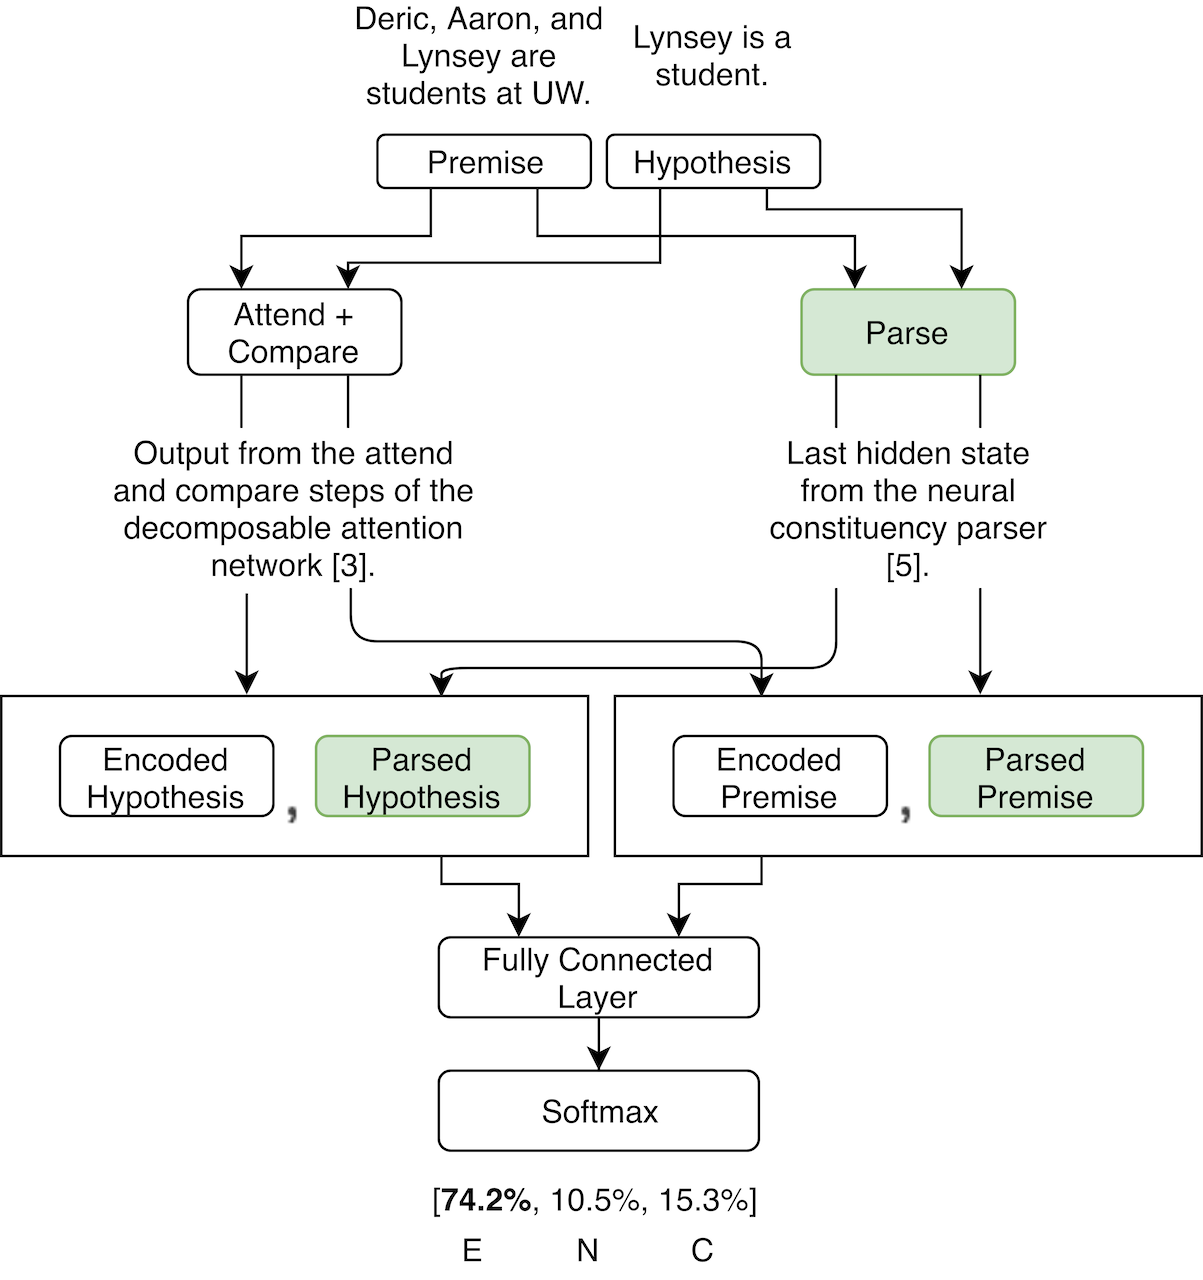
\includegraphics[width=0.45\textwidth]{v1}
%   \caption{A simple method of incorporating syntax into the decomposable
%     attention model.}
% \label{figure:v1}
% \end{figure}


\section{Related Work}

\section{Conclusion}

\bibliographystyle{acl_natbib}
\bibliography{main}

\end{document}
